\documentclass{article}

% set font encoding for PDFLaTeX, XeLaTeX, or LuaTeX
\usepackage{ifxetex,ifluatex}
\if\ifxetex T\else\ifluatex T\else F\fi\fi T%
  \usepackage{fontspec}
\else
  \usepackage[T1]{fontenc}
  \usepackage[utf8]{inputenc}
  \usepackage{lmodern}
\fi

\usepackage{hyperref}

\title{Homework 2}
\author{Marshall Grimmett}

% Enable SageTeX to run SageMath code right inside this LaTeX file.
% http://doc.sagemath.org/html/en/tutorial/sagetex.html
% \usepackage{sagetex}

% Enable PythonTeX to run Python – https://ctan.org/pkg/pythontex
% \usepackage{pythontex}

\usepackage{amsmath}
\usepackage{pgfplots}
\pgfplotsset{compat=1.8}
\usepgfplotslibrary{statistics}

\usepackage{pgfplotstable}
\makeatletter
\long\def\ifnodedefined#1#2#3{%
    \@ifundefined{pgf@sh@ns@#1}{#3}{#2}%
}

\pgfplotsset{
    discontinuous/.style={
    scatter,
    scatter/@pre marker code/.code={
        \ifnodedefined{marker}{
            \pgfpointdiff{\pgfpointanchor{marker}{center}}%
             {\pgfpoint{0}{0}}%
             \ifdim\pgf@y>0pt
                \tikzset{options/.style={mark=*, fill=white}}
                \draw [densely dashed,blue] (marker-|0,0) -- (0,0);
                \draw plot [mark=*] coordinates {(marker-|0,0)};
             \else
                \tikzset{options/.style={mark=none}}
             \fi
        }{
            \tikzset{options/.style={mark=none}}
        }
        \coordinate (marker) at (0,0);
        \begin{scope}[options]
    },
    scatter/@post marker code/.code={\end{scope}}
    }
}

\makeatother

\begin{document}
\maketitle


\section{Part 1}
I started with the initial values of psi and epsilon, but I was only
achieving 1 epoch, so I slowly decreased my epsilon until the number of epochs
was around 5. This way I could find a breaking point for psi and epsilon.
This is because if the psi value is too small then the difference between
epochs will be small as well. I landed on an epsilon value of 0.5 with
the initial psi value of 0.1. The results are below. The y-axis is the
cross entropy error and the x-axis is the number of epochs.

\begin{figure}[h!]
  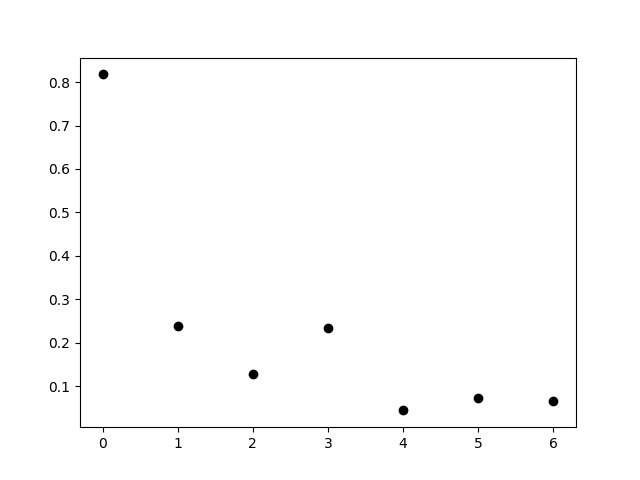
\includegraphics[width=\linewidth]{psi_0.1_epsilon_0.5.png}
\end{figure}

Training average cross entropy error: 0.0001375 \\
Testing average cross entropy error: 2.92e-14 \\

Next, I used psi of 0.01 and epsilon of 0.1.

\begin{figure}[h!]
  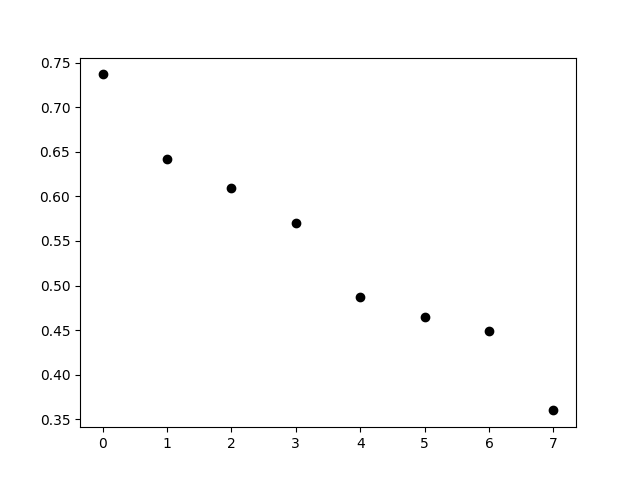
\includegraphics[width=\linewidth]{psi_0.01_epsilon_0.1.png}
\end{figure}

Training average cross entropy error: 0.0007673 \\
Testing average cross entropy error: 9.06e-10 \\

This got much worse, so I decided to increase psi.
I used psi=0.2 and epsilon=0.1

\newpage

\begin{figure}[h!]
  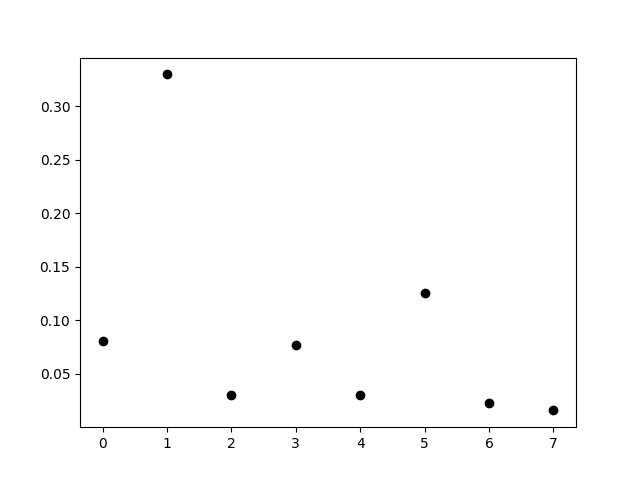
\includegraphics[width=\linewidth]{psi_0.2_epsilon_0.1.png}
\end{figure}

Training average cross entropy error: 3.39e-05 \\
Testing average cross entropy error: 5.33e-17 \\

This obviously got much better. So I decided to test as much as I could
After this and I started getting some errors because the values were
getting too small. So I decided to stick with my final values from the
previous test. In conclusion, a larger step size will make the error
jump around a lot more, while a smaller step size has a steady decrease.
However, a smaller step size will not converge as quickly. A larger epsilon
will oftern make the algorithm stop too soon, and not allow it to discover
better optimal values. While too small of an epsilon will never be reached
and cause us to miss potentially optimal values.


\section{Part 2}


\subsection{a}
Here is the new redesigned MLP with no hidden layer. It consists of
just a single input layer and a single output layer.

\newpage

\begin{figure}[h!]
  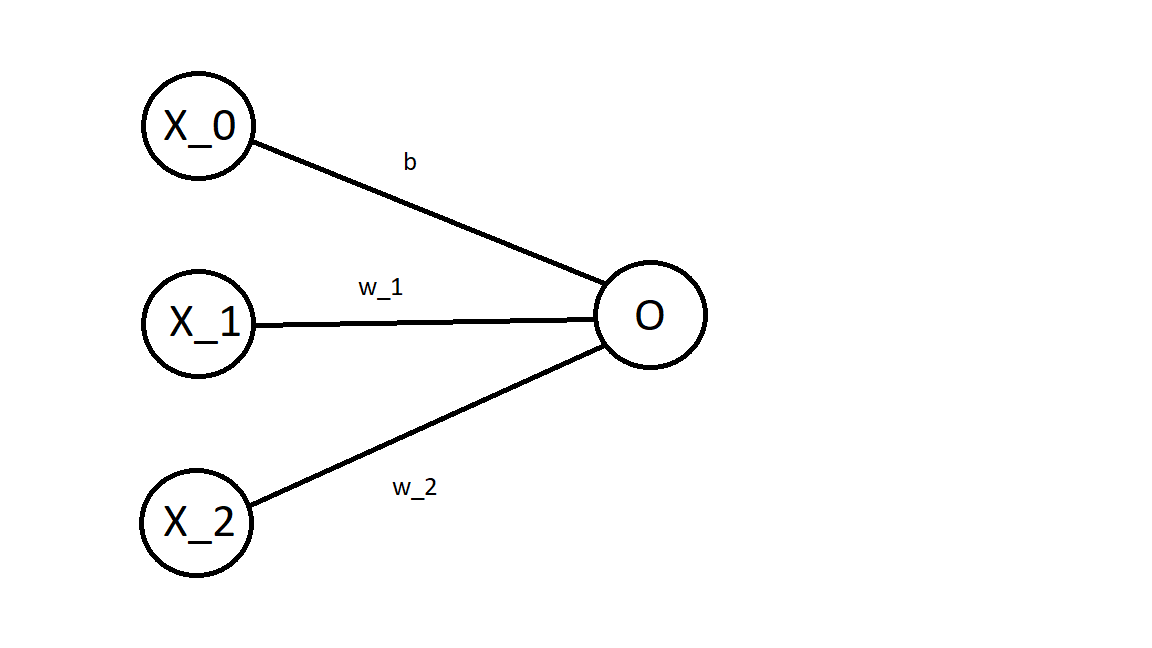
\includegraphics[width=\linewidth]{NewNeuralNet.png}
\end{figure}

We can use the old weights to calculate the new weights
by substitution. \\

Since we are using a linear activation function, the output of unit $j$
in the hidden layer is,
\begin{equation*}
  z_j=c\times(w_j^{h^T}\bar{x})=c\times(\sum_{i=1}^{n}w_{ij}^hx_i+
  b_{j}^hx_0)
\end{equation*}
where $\bar{x}$ is the augmented input vector for some fixed constant scalar
c. \\

More specifically, our $z_1$ will be,
\begin{equation*}
  z_1=c\times((w_{11}^hx_1+b_1^hx_0)+(w_{21}^hx_2+b_1^hx_0)) \\
  =c\times(w_{11}^hx_1+w_{21}^hx_2+2b_1^hx_0)
\end{equation*}
And similarily, our $z_2$ will be,
\begin{equation*}
  z_2=c\times(w_{12}^hx_1+w_{22}^hx_2+2b_2^hx_0)
\end{equation*}

The output of unit $j$ in the output layer is,
\begin{equation*}
  o_j=c\times(w_j^{o^T}\bar{z})=c\times(\sum_{i=1}^{n}w_{ij}^oz_i+
  b_{j}^oz_0)
\end{equation*}
where $\bar{z}$ consists of each neuron in the hidden layer
for some fixed constant scalar c. \\

Similar to above from $z_j$ we can compute $o_j$
\begin{equation*}
  o_1=c\times(w_{11}^oz_1+w_{21}^oz_2+2b_1^oz_0)
\end{equation*}

Since we have no need for the bias term anymore, we
can remove it from the equation.
\begin{equation*}
  o_1=c\times(w_{11}^oz_1+w_{21}^oz_2)
\end{equation*}

Now we just have to substitute in for $z_1$ and $z_2$
and find the new weights.
\begin{multline*}
  o_1=c\times(w_{11}^oz_1+w_{21}^oz_2) \\
  =c\times(w_{11}^o(c\times(w_{11}^hx_1+w_{21}^hx_2+2b_1^hx_0))+
  w_{21}^o(c\times(w_{12}^hx_1+w_{22}^hx_2+2b_2^hx_0))) \\
  =c^2\times((w_{11}^ow_{11}^hx_1+w_{11}^ow_{21}^hx_2+2w_{11}^ob_1^hx_0)+
  (w_{21}^ow_{12}^hx_1+w_{21}^ow_{22}^hx_2+2w_{21}^ob_2^hx_0)) \\
  =c^2\times((w_{11}^ow_{11}^h+w_{21}^ow_{12}^h)x_1+
  (w_{11}^ow_{21}^h+w_{21}^ow_{22}^h)x_2+(2w_{11}^ob_1^h+2w_{21}^ob_2^h)x_0)
\end{multline*}

Thus the new weights and bias term are
\begin{equation*}
  b=2w_{11}^ob_1^h+2w_{21}^ob_2^h=2w_1^{o^T}b_1^h
\end{equation*}
\begin{equation*}
  w_1=w_{11}^ow_{11}^h+w_{21}^ow_{12}^h=w_1^{o^T}w_1^h
\end{equation*}
\begin{equation*}
  w_2=w_{11}^ow_{21}^h+w_{21}^ow_{22}^h=w_1^{o^T}w_2^h
\end{equation*}


\subsection{b}
Yes it is always possible to represent a neural network that only uses
linear neurons without a hidden layer. If you add more neurons to each
layer it will not affect the final solution as above, there will only be
more weights, but the dot product will remain the same. If you add more layers,
then we can think of our new weights as the input for another layer, making
our output layer into a hidden layer. So then we just repeat the process,
using our new weights to substitute into the new output layer. For example,
our new weights from the final equations, would become the vector $w_1^h$.
I.e. $w_1^h=[w_1,w_2]^T$. There will likely be other neurons added to this
layer, which is why I chose $w_1^h$, I could have also chosen $w_2^h$.


\end{document}
